%
% Complete documentation on the extended LaTeX markup used for Insight
% documentation is available in ``Documenting Insight'', which is part
% of the standard documentation for Insight.  It may be found online
% at:
%
%     http://www.itk.org/

\documentclass{InsightArticle}


%%%%%%%%%%%%%%%%%%%%%%%%%%%%%%%%%%%%%%%%%%%%%%%%%%%%%%%%%%%%%%%%%%
%
%  hyperref should be the last package to be loaded.
%
%%%%%%%%%%%%%%%%%%%%%%%%%%%%%%%%%%%%%%%%%%%%%%%%%%%%%%%%%%%%%%%%%%
\usepackage[dvips,
bookmarks,
bookmarksopen,
backref,
colorlinks,linkcolor={blue},citecolor={blue},urlcolor={blue},
]{hyperref}
% to be able to use options in graphics
\usepackage{graphicx}
% for pseudo code
\usepackage{listings}
% subfigures
\usepackage{subfigure}


%  This is a template for Papers to the Insight Journal. 
%  It is comparable to a technical report format.

% The title should be descriptive enough for people to be able to find
% the relevant document. 
\title{FFT shift}

% Increment the release number whenever significant changes are made.
% The author and/or editor can define 'significant' however they like.
% \release{0.00}

% At minimum, give your name and an email address.  You can include a
% snail-mail address if you like.
\author{Ga\"etan Lehmann}
\authoraddress{INRA, UMR 1198; ENVA; CNRS, FRE 2857, Biologie du D\'eveloppement et
Reproduction, Jouy en Josas, F-78350, France}

\begin{document}
\maketitle

\ifhtml
\chapter*{Front Matter\label{front}}
\fi


\begin{abstract}
\noindent
% The abstract should be a paragraph or two long, and describe the
% scope of the document.

A common usage when working with Fourier transform is to shift the
the image to put the zero-frequency component in the center of the
image. This contribution comes with a filter to perform this
transform.
\end{abstract}

% \tableofcontents

This filter is multitreaded and works with any dimensions or size of image.

When the size of the image is odd on one dimension or more, performing the
transform twice will not produce the same image than the input, as shown in
the figure below. To get it right, the option \verb$SetInverse(true)$ has
to be used.

The filter is very simple, and there shouldn't be any problem to use it. Please
look at check.cxx in the tar ball for an example.

\begin{figure}[htbp]
\centering
\subfigure[input image]{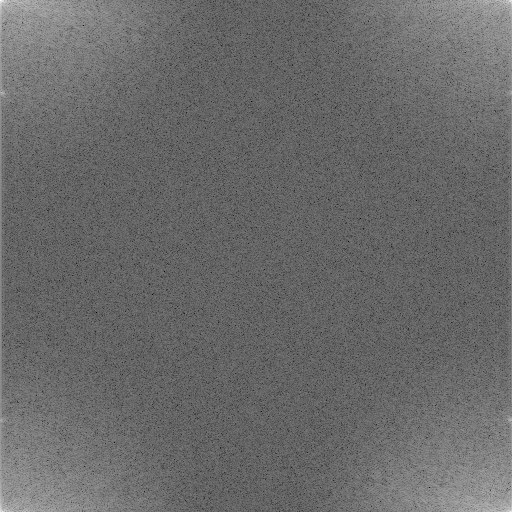
\includegraphics[scale=0.4]{fft}}
\subfigure[shifted image. The zero components are now centered.]{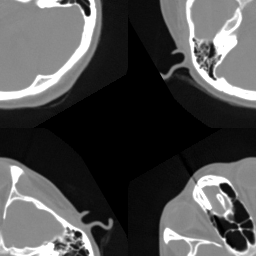
\includegraphics[scale=0.4]{test}}
\caption{Result of the transform on the log of the modulus of the fft transform of a real image.}
\end{figure}

\begin{figure}[htbp]
\centering
\subfigure[input image]{\includegraphics[scale=15]{5X5}}
\subfigure[shifted image, with Inverse = false]{
\includegraphics[scale=38.1]{shifted5X5}}
\subfigure[the image shifted twice, with Inverse = false for the first run, and Inverse = true for the second]{\includegraphics[scale=15]{5X5}}
\subfigure[the imageshifted twice, with Inverse = false for both the first and the second run. The input image is not restored.]{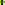
\includegraphics[scale=38.1]{nonInverse5X5}}
\caption{Result of the transforms on an image with an odd size (5x5).}
\end{figure}

\appendix



\bibliographystyle{plain}
\bibliography{InsightJournal}
\nocite{ITKSoftwareGuide}

\end{document}

